% !TEX root = MAIN.tex

\subsubsection{Background - SEMu}
\label{klee-semu}

\STARTCHANGEDWPT

SEMu~\cite{chekam2021killing} is a mutant analysis  framework based on dynamic symbolic execution that has been built on top of the KLEE Symbolic Virtual Machine~\cite{cadar2008klee}.

\TODO{Add reference for differential symbolic execution}
SEMu uses a form of differential symbolic execution~\cite{} to generate test inputs that kill mutants. The approach consists of modeling the mutant killing problem as a symbolic execution search in a scalable and cost-effective way. 
The SEMu framework is the building block of 
%act as a baseline for 
the test generation tool developed in FAQAS (i.e., \emph{SEMuS}, see Section~\ref{sec:semus}).

To kill a mutant, we need test cases that capture the three killing conditions of a mutant~\cite{offutt1997automatically}: 
\begin{itemize}
	\item \textbf{reachability}: the test case should execute the mutated statement
	\item \textbf{necessity}: the test case should cause an incorrect intermediate state, if it reaches the mutated statement
	\item \textbf{sufficiency}: the final state of the mutated program should differ from the one of the original program
\end{itemize}

\TODO{the concept of "mutation point is not clear"; you do not clarify that the two versions are compiled in the same executable}
The technique works by executing both the original program and mutant program through symbolic execution, where the mutant executions fork every time it reaches a mutation point. 
\TODO{not clear that the forked execution concerns the mutant}
\TODO{"compares with it" does not have a meaning; also, what is a state here?}
The forked execution follows the original execution and compares with it at each state. 
\TODO{what does it mean "differentially compare"?}
The technique differentially compares the symbolic states of the two executions, forked and original, and generate test inputs. 

\begin{figure}[tb]
\begin{center}
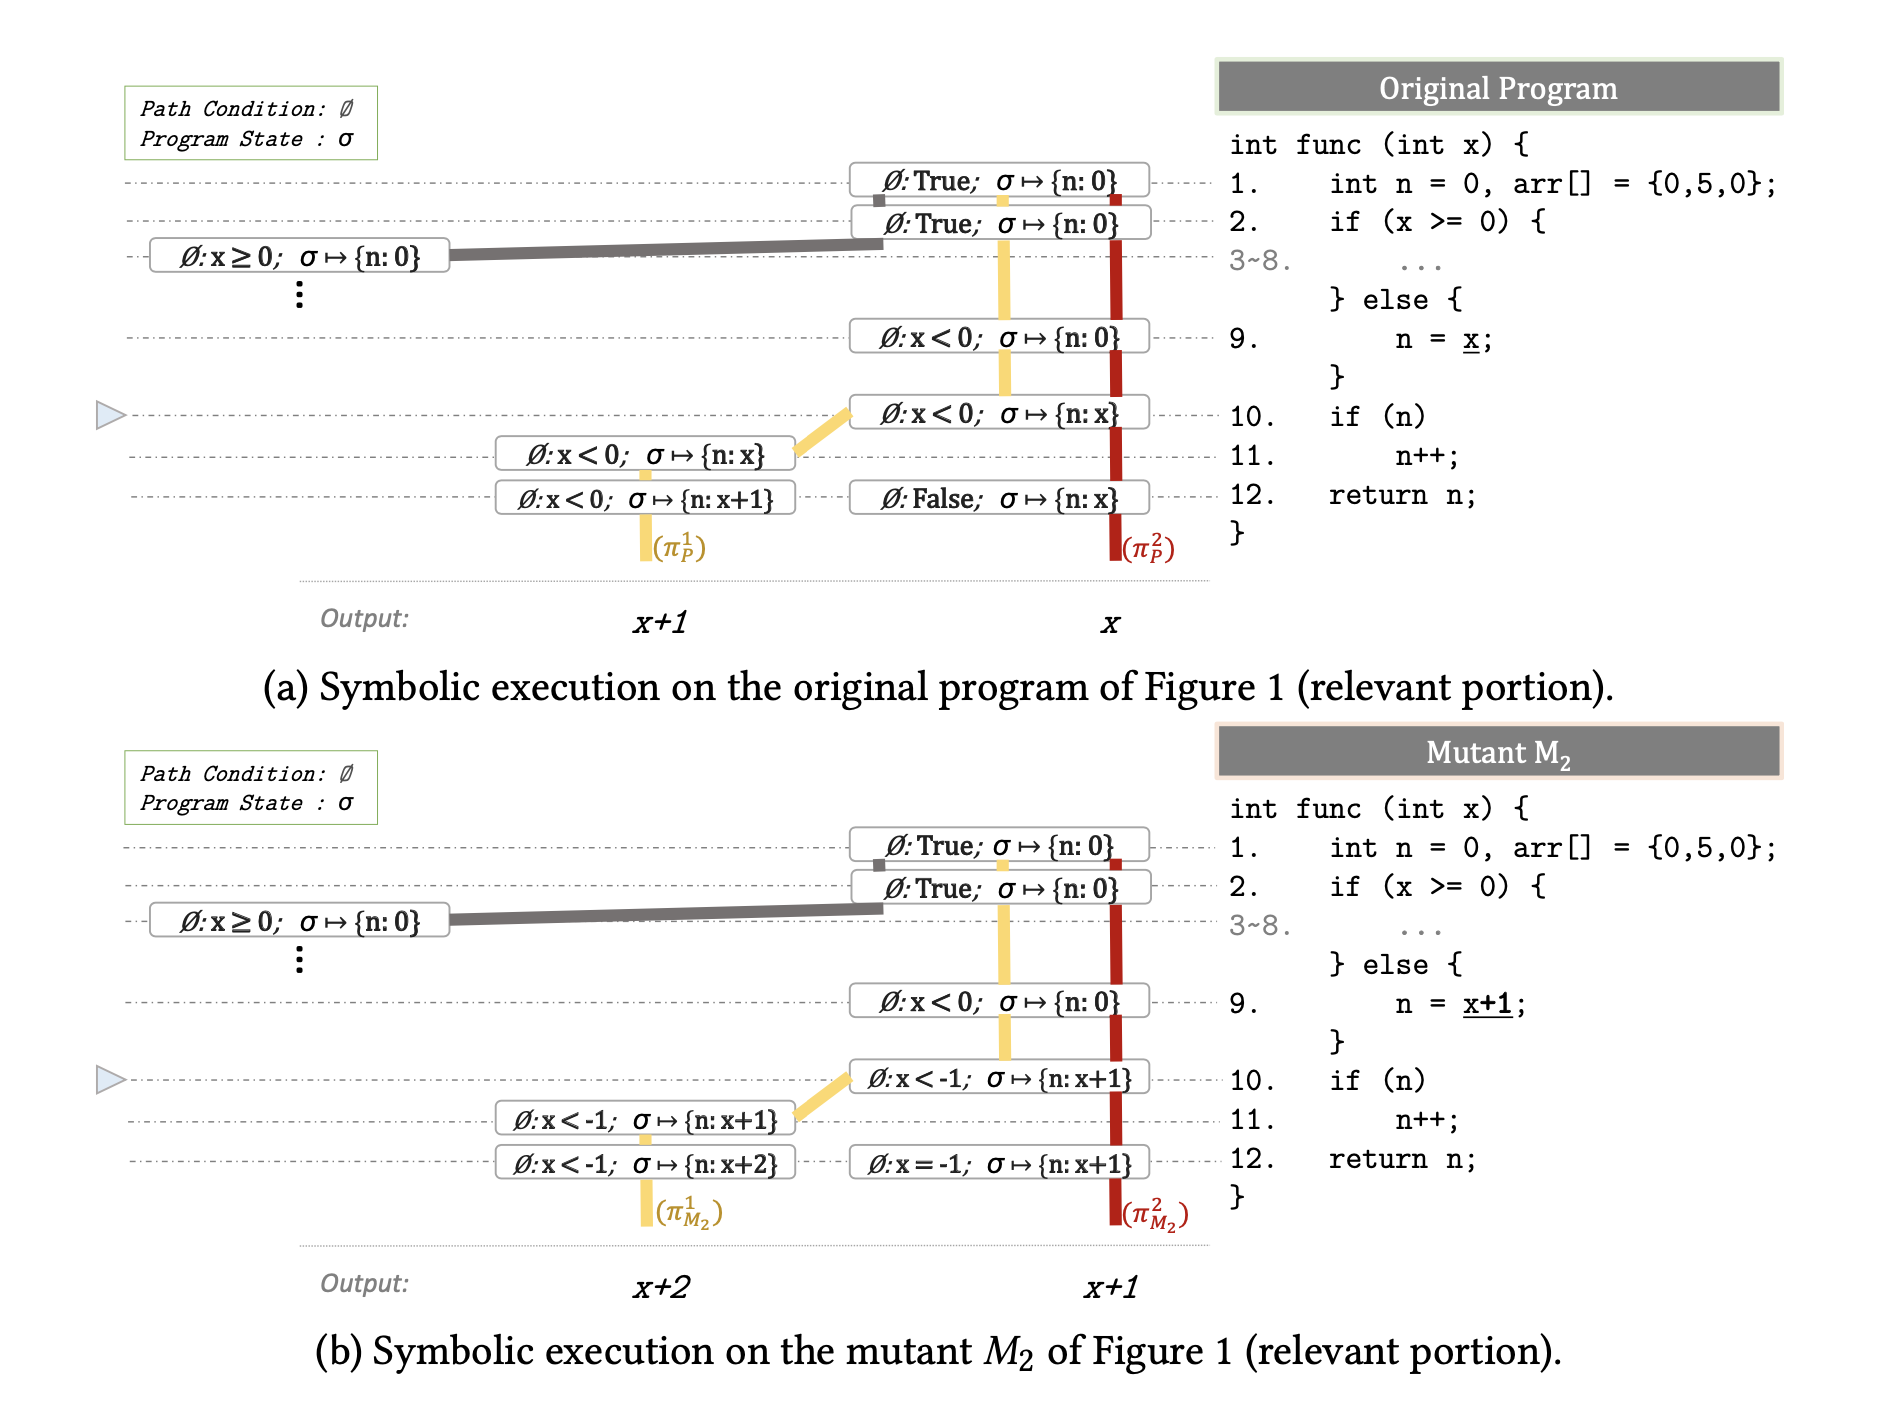
\includegraphics[width=\textwidth]{images/semu-example}
\caption{SEMu example. Source: Chekam et al.~\cite{chekam2021killing}.}
\label{fig:semu-example}
\end{center}
\end{figure}

Figure~\ref{fig:semu-example} introduces an example of dynamic symbolic execution, sub-figure (a) shows the symbolic execution for the original program, while (b) shows the symbolic execution process for the mutant version. In order to generate test inputs that kill a mutant, the technique applies symbolic execution to a program $P$ and to its respective mutant $M_2$, to produce their respective symbolic paths. In a second step, the technique solves the formula $kill(\pi_P, \pi_{M_2})$ to generate the test inputs that kills $M_2$ and goes through $\pi_P$ in $P$ and through $\pi_{M_2}$ in $M_2$. 

As shown in Figure~\ref{fig:semu-example}, symbolic execution on the original program leads to the paths $x < 0$ and $False$, with the respective outputs $x + 1$ and $x$.
Instead, the symbolic execution on the mutant leads to paths $x < -1$ and $x = -1$, with outputs $x + 2$ and $x + 1$.

Consequently, the only feasible path that targets mutant $M_2$ is the following:

\begin{equation}
	kill(\pi_{P}^{1}, \pi_{M_2}^{1}) = ((x < 0) \wedge (x + 1 \neq x + 2) )
\end{equation}

Where the solution to $kill(\pi_{P}^{1}, \pi_{M_2}^{1})$ is $x = -2$.

The symblic execution process introduced above is largely inefficient; indeed,
%However, the problem of this approach is that 
(1) it requires a complete symbolic execution on $P$ and on each mutant $M$, (2) all path conditions and symbolic outputs have to be stored, and (3) all kill formulas has to be solved for each pair of paths conditions. 
%This scenario leads to high execution costs making the approach impractical.
For this reason, SEMu introduces a list of optimizations to reduce execution time:

\begin{itemize}
	\item \textbf{Meta-mutation}: all mutants are encoded into a single program (in FAQAS, we extended it at source code level), the mutant is selected through a branching statement named mutant choice statement.
	\item \textbf{Discarding non-infected mutant paths}: mutant paths failing to infect the program state are discarded immediately.
	\item \textbf{Heuristic search}: stop exploration of a path after $K$ transitions, and solve the kill formula.
	\item \textbf{Infection-only strategy}: Generates test inputs by aiming only at mutant infection.
\end{itemize}

\TODO{I have the impression that none of the following heuristics are currently used in FAQAS. I would write that we indicate which heuristics are not feasible and which one may be investigated in follow-up activities.}
To reduce execution time further, SEMu also introduces a list of parametric heuristics that can be controlled by the user; this set of heuristics help to define which paths to explore and in general, the test generation process:

\TODO{please use "test cases" not "tests"}
\begin{itemize}
	\item \textbf{Controlling for reachability} (seeded symbolic execution): explore paths in seeded  mode up to a given length. 
	\TODO{You are not explained what t does. "This heuristic consists of executing the original program up to a given path using the same inputs provided by existing test cases; it generates symbolic inputs only for...  For its implementation SEMu relies on a feature provided by KLEE"}
	This heuristic quickly prunes paths that are infeasible or does not reach the mutant. 
	\TODO{Please refine what I wrote in the following. You were not explicitly clrifying hat the problem is.}
	We do not integrated this feature in FAQAS because of two reasons. First, SEMu can deal only with test cases for batch programs (i.e., providing arguments to the main function of the software under test), which is different from our context where we either have unit or integration test cases implemented in a programming language or we have complex system test cases simulating communication from ground to orbit through network and a simulator. Second, in our context, because of the complexity of the SUT we can generate unit test cases but not integration or system level ones. The main difference between such test cases is the entry point, for unit test cases it is the function under test, for integration or system test cases it is a function different than the function under test. Consequently, implementing such solution would require the implementation of additional technology to map the seeds collected for test inputs with different entry points, which is not provided by KLEE.

	\item \textbf{Controlling for propagation}: sometimes an infected program state fails to propagate the infection to the outputs, these states should be quickly discarded. 
	\TODO{Rewrite the sentence, unclear}
	For the propagation four heuristic parameters are introduced:
	\begin{itemize}
	\item \TODO{(Comments are put above the problematic item) Unclear. Do you want to say that it consider checkpints with a predefined distance? Pleas write complete sentences sbject-verb-object.}
		\item \textbf{Checkpoint Window}: determines the distance between checkpoints (program location with branching statements). 
		\TODO{What are the criteria to discard a branch?}
		At every checkpoint (1) some branches are discarded, (2) generate tests based on the current states. Not used in FAQAS because we deal with unit testing (i.e., we test the mutated function).
		\TODO{There is no more time for investigation, no? Explain why we discard it then.}
		\item \textbf{Propagating Proportion}: specifies the percentage of branches that are kept to pursue the exploration. To be investigated in FAQAS.
		\TODO{You write "these branches", which branches? If all teh heuristics concern finding branches you need to specify above.}
		\TODO{To be investigated no}
		\item \textbf{Propagation Selection Strategy}: determines how these branches are selected, it can be done (1) randomly, or (2) selecting the branch that is closer to the output. Even though, the random strategy works better with batch programs according to literature~\cite{chekam2021killing}, we deal with unit tests for large programs. To be investigated in FAQAS. 
		\TODO{Why}
	\item \textbf{Minimum Propagation Depth}: how many checkpoints should pass before generating the tests. Not used in FAQAS.
	\end{itemize}

	\TODO{Do not require for dong what? Complete the sentence. Who is the subject?}
	\item \textbf{Controlling the cost of constraint solving} (no state difference): do not require the state of the original program to be different from the mutant. Not used in FAQAS.

	\TODO{Unclear. Who is the subject?}
	\item \textbf{Controlling the number of attempts} (number of tests per mutant): specifies the number of tests to be generated for each mutant. Based on the idea that a test can kill multiple mutants. To be investigated in FAQAS (for now, we generate only one mutant a time).

\end{itemize}

\ENDCHANGEDWPT

